\documentclass[../mathNotesPreamble]{subfiles}
\begin{document}
%\relscale{1.4}
\section{3.3: Rules of Differentiation}
\begin{thmBox*}[Theorem 3.2: Constant Rule]
  If $c$ is a real number, then $\dfrac{d}{dx}(c)=0$.
\end{thmBox*}

\begin{ex*}
  Find the derivatives of
  \begin{tasks}(3)
    \task[] $f(x)=3$ \task[] $g(x)=\pi$ \task[] $h(x)=e^\pi$
  \end{tasks}
\end{ex*}
\vspace*{\stretch{1}}

\begin{thmBox*}[Theorem 3.3: Power Rule]
  If $n$ is a nonnegative integer, then $\dfrac{d}{dx}\parens{x^n}=nx^{n-1}$
\end{thmBox*}

\begin{ex*}
  Find the derivative of 
  \begin{tasks}(3)
    \task[] $j(x)=x^3$
    \task[] $\ell(x)=x^\pi$
    \task[] $m(x)=\pi^{42\cos(e)}$
  \end{tasks}
\end{ex*}
\vspace*{\stretch{1}}
\pagebreak

\begin{proof}(Briggs, p153)

  Let $f(x)=x^n$ and use the definition of the derivative in the form
    $$f'(a)=\lim_{x\to a}\dfrac{f(x)-f(a)}{x-a}$$

  With $n=1$ and $f(x)=x$, we have
    $$f'(a)=\lim_{x\to a} \dfrac{f(x)-f(a)}{x-a}=\lim_{x\to a} \dfrac{x-a}{x-a}=1$$

  as given by the Power Rule.
 
  With $n\geq 2$ and $f(x)=x^n$, note that $f(x)-f(a)=x^n-a^n$. A factoring formula gives
    $$x^n-a^n=(x-a)(x^\nmo+x^\nmo[2]a+\dots+xa^\nmo[2]+a^\nmo).$$

  Therefore,
    \begin{align*}
      f'(a)&=\lim_{x\to a} \dfrac{x^n-a^n}{x-a}\\
        &=\lim_{x\to a} \dfrac{(x-a)(x^\nmo+x^\nmo[2]a+\dots+xa^\nmo[2]+a^\nmo)}{x-a}\\
        &=\lim_{x\to a} (x^\nmo+x^\nmo[2]a+\dots+xa^\nmo[2]+a^\nmo)\\
        &=\underbrace{a^\nmo+a^\nmo[2]\cdot a+\dots+a\cdot a^\nmo[2]+a^\nmo}_{n \text{ terms}}=na^\nmo
    \end{align*}
\end{proof}
\pagebreak

  \begin{thmBox*}[Theorem 3.4: Constant Multiple Rule]
    If $f$ is differentiable at $x$ and $c$ is a constant, then
      $$\dfrac{d}{dx}\parens{cf(x)}=cf'(x)$$
  \end{thmBox*}

\begin{ex*}\ 
  \begin{tasks}(3)
    \task[] $\dfrac{d}{dx}\parens{-4x^9}$
    \task[] $\dfrac{d}{dx}\parens{-\dfrac{7x^{11}}{8}}$
    \task[] $\dfrac{d}{dx}\parens{\frac{1}{3}x^3}$
  \end{tasks}
\end{ex*}
\vspace*{\stretch{1}}

\begin{thmBox*}[Theorem 3.5: Sum Rule]
  If $f$ and $g$ are differentiable at $x$, then 
    $$\dfrac{d}{dx}\parens{f(x)+g(x)}=f'(x)+g'(x)$$
\end{thmBox*}

\begin{ex*}
  Find the derivative of the following:
  \begin{tasks}(2)
    \task[] $p(x)=3x^{100}+4x^e-17x+24-\pi^{\cos(e)}$
    \task[] $t(w)=2w^3+9w^2-6w+4$
  \end{tasks}
\end{ex*}
\vspace*{\stretch{1}}
\pagebreak

\begin{defn*}(The Number $e$)

  The number $e=2.718281828459\dots$ satisfies
    $$\lim_{h\to 0} \dfrac{e^h-1}{h}=1$$

  It is the base of the natural exponential function $f(x)=e^x$
\end{defn*}
\textit{Note:} One way to show the above result is to recall that $\ds\lim_{n\to \infty} \parens{1+\dfrac{1}{n}}^n=e$.
\vspace*{30pt}

\begin{thmBox*}[Theorem 3.6: The Derivative of $e^x$]
  The function $f(x)=e^x$ is differentiable for all real numbers $x$, and 
    $$\dfrac{d}{dx}\parens{e^x}=e^x$$
\end{thmBox*}
\vspace*{20pt}

\begin{proof}
  $$\dfrac{d}{dx}\parens{e^x}
      =\lim_{h\to 0}\dfrac{e^{x+h}-e^x}{h}
      =\lim_{h\to 0} \dfrac{e^x\cdot e^h-e^x}{h}
      =e^x\cdot\lim_{h\to 0} \dfrac{e^h-1}{h}
      =e^x\cdot 1=e^x$$
\end{proof}
\vspace*{20pt}

\begin{ex*}
  Find the derivatives of the following
  \begin{tasks}(3)
    \task[] $e^x$
    \task[] $42e^x$
    \task[] $7e^x-14x^e$
  \end{tasks}
\end{ex*}
\pagebreak

\begin{ex*}
  \textit{Note:} Simplify the expression before taking the derivative
  \begin{tasks}[after-item-skip=\stretch{0.5}](2)
    \task $\dfrac{d}{ds}\parens{\dfrac{12s^3-8s^2+12s}{4s}}$
    \task $h(x)=\dfrac{x^3-6x^2+8x}{x^2-2x}$
    \task $\dfrac{d}{dx}\parens{\dfrac{x-a}{\sqrt x-\sqrt a}}$
    \task $g(w)=\begin{cases}
      w+5e^w,& \text{if }w\leq 1\\
      2w^3+4w+5,& \text{if } w>1
    \end{cases}$
    \task[]
  \end{tasks}
\end{ex*}
\pagebreak

\begin{ex*}
  Use the table to find the following derivatives:
  \begin{center}
  
    \begin{tabular}{@{}L@{\hspace*{15pt}}*{5}{@{\hspace*{25pt}}l}@{}}
      \toprule
      x& 1& 2& 3& 4& 5\\\midrule
      f'(x)& 3& 4& 2& 1& 4\\
      g'(x)& 2& 4& 3& 1& 5\\\bottomrule
    \end{tabular}
  \end{center}
  \vspace*{15pt}
  \begin{tasks}(3)
    \task $\left. \dfrac{d}{dx}\sbrkt{f(x)+g(x)}\right\rvert_{x=1}$
    \task $\left. \dfrac{d}{dx}\sbrkt{1.5f(x)}\right\rvert_{x=2}$
    \task $\left. \dfrac{d}{dx}\sbrkt{2x-3g(x)}\right\rvert_{x=4}$
  \end{tasks}
\end{ex*}
\vspace*{75pt}
\begin{ex*}
  Find the equation of the tangent line to $y=x^3-4x^2+2x-1$ at $a=2$
  \vspace*{\stretch{1}}
\end{ex*}
\begin{ex*}
  Find the equation of the tangent line to $y=\dfrac{e^x}{4}-x$ at $a=0$.
  \vspace*{\stretch{1}}
\end{ex*}
\pagebreak

\begin{ex*}
  Find the equation of the normal line to $f(x)=1-x^2$ at $x=2$.
  \vspace*{\stretch{1}}
\end{ex*}
\begin{ex*}
  Find the equations of the tangent line and normal line to $y=\dfrac{1}{2}x^4$ at $a=2$.
  \vspace*{\stretch{1}}
\end{ex*}
\begin{ex*}
  At what $x$-values does $f(x)=x-2x^2$ have horizontal tangents?
  \vspace*{\stretch{1}}
\end{ex*}
\pagebreak

\begin{ex*}
  Find an equation of the line having slope $\dfrac{1}{4}$ that is tangent to the curve $y=\sqrt x$.
  \vspace*{\stretch{1}}
\end{ex*}
\begin{ex*}\ 

  \noindent
  \begin{minipage}{0.45\linewidth}
    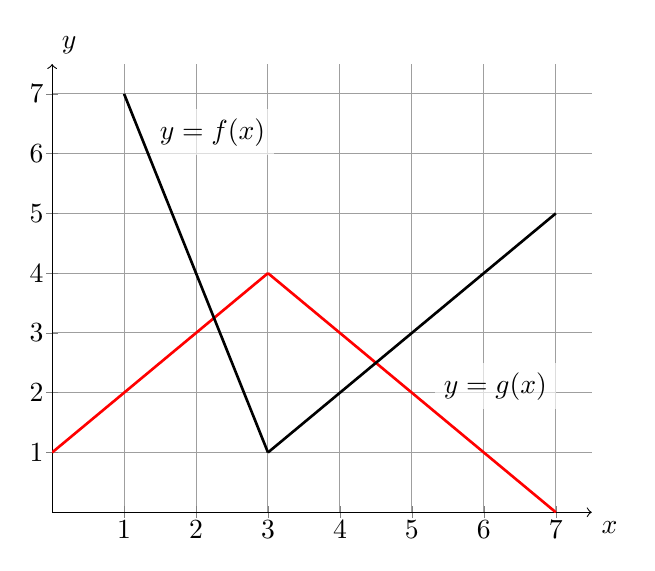
\begin{tikzpicture}
      \begin{axis}[
        grid=both,
        grid style={line width=0.35pt, draw=gray!75},
        axis lines=center,
        axis line style={->},
        xmin=0, xmax=7.5,
        ymin=0, ymax=7.5,
        xtick={0,1,...,7},
        ytick={0,1,...,7},
        ticklabel style={font=\normalsize, inner sep=0.75pt,fill=white,opacity=0.65, text opacity=1},
        xlabel=$x$, xlabel style={at={(ticklabel* cs:1)},anchor=north west},
        ylabel=$y$, ylabel style={at={(ticklabel* cs:1)},anchor=south west},
        every axis plot/.append style={line width=0.95pt}
        ]
        \addplot[-] expression[domain=0:3, red]{x+1};
        \addplot[-] expression[domain=3:7, red]{-x+7} node[above right, black, pos=0.575,  fill=white, opacity=0.65, text opacity=1] {$y=g(x)$};
        \addplot[-] expression[domain=1:3]{-3*x+10} node[above right, black, pos=0.175,  fill=white, opacity=0.65, text opacity=1] {$y=f(x)$};
        \addplot[-] expression[domain=3:7]{x-2};
      \end{axis}
    \end{tikzpicture}
  \end{minipage}%
  \begin{minipage}{0.55\linewidth}
    \begin{tasks}[after-item-skip=25pt](1)
      \task $f'(2)$
      \task $g'(2)$
      \task $f'(5)$
      \task $g'(5)$
    \end{tasks}
  \end{minipage}
\end{ex*}
\pagebreak
\begin{ex*}
  The line tangent to the graph of $f$ at $x=5$ is $y=\dfrac{1}{10}x-2$. Find $\left.\dfrac{d}{dx}\parens{4f(x)}\right\rvert_{x=5}$
  \vspace*{\stretch{1}}
\end{ex*}
\begin{ex*}
  At what point on the curve $y=1+2e^x-3x$ is the tangent line parallel to the line $3x-y=5$.
  \vspace*{\stretch{1}}
\end{ex*}
\begin{ex*}
  Find equations of both lines that are tangent to the curve $y=1+x^3$ and parallel to the line $12x-y=1$.
  \vspace*{\stretch{1}}
\end{ex*}
\pagebreak
\begin{defn*} Higher-Order Derivatives

  Assuming $y=f(x)$ can be differentiated as often as necessary, the \textbf{second derivative} of $f$ is
    $$f''(x)=\dfrac{d}{dx}\parens{f'(x)}$$
    
  For integers $n\geq 1$, the \textbf{$\bm n$th derivative} of $f$ is
    $$f^\parens{n}(x)=\dfrac{d}{dx}\parens{f^\parens{\nmo}(x)}$$
\end{defn*}
\vspace*{20pt}
\begin{ex*}
  Find all the derivatives of $y=\dfrac{x^5}{120}$
  \vspace*{\stretch{1}}
\end{ex*}
\begin{ex*}
  Find the first, second and third derivatives of $f(x)=5x^4+10x^3+3x+6$
  \vspace*{\stretch{1}}
\end{ex*}
\begin{ex*}
  Find the first, second and third derivatives of $f(x)=x^2\parens{2+x\inv[3]}$.
  \vspace*{\stretch{1}}
\end{ex*}
\pagebreak
\end{document}
